% arara: lualatex: {shell: 1}
%!TeX TS-program=arara
\documentclass{article}
%\input{../pre.tex}
\usepackage{fontspec}
\usepackage[T1]{fontenc}
\usepackage{mathpazo}
\usepackage[inline]{enumitem}
\usepackage{tabu}
\usepackage{booktabs}
\usepackage{hyperref}
\usepackage{amsmath}
\usepackage{amssymb}
\usepackage{amsthm}
\usepackage{xfrac}
\usepackage{nth}
\usepackage{minted}
%\usepackage[nomarkers,figuresonly]{endfloat}
\setmonofont[Scale=MatchLowercase,Contextuals={Alternate}]{FuraCode Nerd Font}
\setminted{frame=lines,framesep=1em,fontsize=\small}

\title{Fractal Patterns and Music}
\date{MATH-538, December 2019}
\author{Javier, Chris Benito, Nils Olsson}

\begin{document}
\maketitle

\section{Abstract}

In this paper we explain the current state of fractals in music. We
include a description of fractals and how they can be perceived in music. We
discuss how the note frequencies follow a power law relation across many genres
of western music. We present the Michael Bulmer’s technique for creating music
that is close to true pink noise. There is also an overview of how fractals have
occurred in musical compositions in the past, including the specific example in
Bach’s Cello Suite No. 3. Then we created a program to perform dimension
calculations of music.

\section{Fractals}

Out of principle we must begin our discussion on fractals in music by mentioning
the late Benoit Mandelbrot. Mandelbrot coined the phrase “fractal” in 1975 to
describe objects that retained complexity and detail, at different scales;
similar to how the photograph of a pile of rocks can look similar to the picture
of a mountain, if there is nothing to provide a sense of scale\cite{3}. Initially,
Mandelbrot observed this in time series graphs of product prices in the economy,
where if there was no scale it would be impossible to tell if the price changes
were updated per minute, hour, day, etc.\cite{3}. Mandelbrot also tended to speak of
“roughness”\cite{4}. Something that was smooth would be akin to time series plot that
looked like a smooth curve. A rough graph would look like a plot with many
dynamic changes.

Mandelbrot believed in the power of the human eye to notice
“roughness”\cite{3,4}, but music provides a unique challenge, because in the
moment, music is felt in a psychological sense, and is usually not observed as a
whole, unless one acquires sheet music or other physical interpretation of the
music as the composer intended. In fact, in the memoir Benoit Mandelbrot A life
in Many Dimensions, Harlan Brothers wrote, “Benoit Mandelbrot always had a
strong feeling that music could be viewed from a fractal perspective. However,
without our eyes to guide us, how do we gain this perspective?”[ALMD] The
question posed is an excellent one, and Brothers goes on to discuss that
generally there are seven ways that fractals can appear in music.

Before we discuss these seven ways, we would like to mention that there are
several misconceptions as to what fractal music is of which Brothers discusses\cite{5}.
The most common misconception is that converting fractal images into sound
produces fractal music. In many cases these transformations can hardly be
classified as music and simply as noise. Another misconception is to think that
iterations always cause fractals in music. This is not true in the physical
sense as the logistic map illustrates\cite{5} and it does not hold in music either.
The last misconception that Brothers talks about in regard to fractal music is
that of self-similarity. As with fractal diagrams, self-similarity is a
necessary but not sufficient condition\cite{5}. He gives the example that, “ onions,
spirals, and Russian dolls are not fractal; they do not contain a minimum of two
matching or similar regions in which the arrangement of elements either mirrors
or imitates the structure of the object as a whole.”\cite{5}. So, it is necessary
that parts of a musical piece be similar to larger sections of the musical
composition.

\section{A primer on music}

Before introducing the different ways in which fractal patterns arise in music
it is essential that some basic building-blocks of music be introduced.

\subsection{Pitch, intervals, and rhythm}

A single key on a piano, when struck, produces a single pitch. Pitch is one of
the most fundamental properties of notes in music, but what exactly is pitch?
The sound that is produced by the piano is really the combination of several
strings vibrating, each producing different frequencies of sound. Together this
combination forms the characteristic sound of the piano (also called timbre, the
specific quality to the sound of, in this case, the piano). The strongest
frequency in this collection is called the fundamental frequency of the “note”
being played, and to this frequency a name is assigned. In the case of a piano,
and of all Western music, these frequency names come from the alphabet: A, B, C,
D, E, F, and G. Though pitches are unique unto their frequency, some pitches are
considered equivalent with respect to the ratio of their frequencies. For
example, the pitch A4 (concert A) sounds at 440 cycles per second (hertz), while
A5 sounds at 880 hertz: a ratio of 1:2. This ratio is called an octave, and thus
we have names for distances between frequencies which we call intervals. Within
Western music notation there are a finite number of named intervals; here’s a
few: perfect octaves, perfect fifths, diminished fifths, augmented fourths
(equivalent to diminished fifths), major thirds, minor thirds, etc. Between any
two notes (and even between a note and itself) there is an interval between
them, and is measured aptly by counting the number of keys of the piano it takes
to get from one note to the other where these steps are called “semitones”. For
example, the interval between any F and the nearest B on the piano consists of
six semitones. As an aside, this interval is known as a tritone and is one of
the most dissonant intervals producible on the piano. Returning to octaves,
despite having unique frequencies, any two pitches which are an interval of an
octave apart (or multiple octaves apart, e.g. C2 and C5) from one another, are
considered equivalent. Lastly, If you are familiar with the piano then you will
know there are actually are more than seven keys in between octaves, twelve
precisely. These are just smaller subdivisions of the frequency ranges between
octaves.

The other most fundamental property of notes is duration, also called rhythmic
value (or simply “value”). Music as listened to is inherently ephemeral: in the
moments in which we experience music by listening to it, it exists, but then it
is gone. How long we experience the sound of a pitch is called its duration, and
we might measure the duration of a pitch by how long it is played in seconds.
Establishing a baseline duration is important in the composition of music; some
pieces of music consist of pitches that are long in duration, while others
consist of pitches that exist only for a split-second. But not all pitches need
have the same duration, and so we have rhythm: the ratios between pitches in
terms of duration. For example we might play one pitch for twice as long as the
one before, and the next two pitches for a quarter as long. Like with pitch,
different rhythmic values also have names within Western music notation, some of
the most basic of which being whole notes, half notes, quarter notes ♩, and
eighth notes ♪. Notice that the names all have to do with fractions. A piece of
music might set a baseline speed by stating that the duration of a quarter note
should be a certain number of seconds—then the duration of a half note would be
twice as long as the duration of the quarter note, a whole note four times as
long, an eighth note half as long, a sixteenth note a quart as long, etc.
It is these two fundamental properties that are a part of every note in a piece of music.

\subsection{Melody and harmony}

Melody and harmony are in some ways the two sides to a coin: melody is how notes
move one at a time in a single line horizontally across the page, while harmony
is how notes sound simultaneously. Colloquially we call harmony the experience
of multiple things working together in tandem in a pleasing manner. In music,
“working in tandem” might mean how “good” two or more notes sound together. The
notes C E and G played simultaneously form a kind of harmony that is familiar to
anyone that is accustomed to Western music: a C major chord. Chords similar to
this one are characterized often emotively, but also intervalically (that is by
ratios of the distances between the notes forming the chord), and since it is
hard to quantify emotion, analysis of music usually pertains to intervals.
Melodic analysis pertains to observing the intervals between sequential notes
that are not simultaneous. Just as before, the notes C E and G form a C major
chord, but if played sequentially instead of simultaneously we have melody
instead of harmony and possibly a different emotional experience altogether
(this breaking up of harmony is called arpeggiation).

\section{Self-similarity scaling in music}

As a subject of research, fractals and self-similarity in music may be fairly
niche, but there is no shortage of literature, new or old. One of the earliest
attempts at mathematically quantifying musical self-similarity was conducted by
Richard Voss and John Clarke, and in 1975 they published the article ``$\sfrac 1
f$ noise in music and speech''. They concluded that, within genres of music, a
$\sfrac 1 f$ power-law scaling behavior is characteristic of musical components
for pieces in the genre (though they were specifically concerned with the
Baroque era compositions of J.S. Bach, or just ``classical'' in layman's terms).

However, there may be many different ways in which measurable self-similarity
within music can manifest; chapter 7 of the Mandelbrot text, written by
Brothers, provides a few examples of how scaling within music has been
quantified:

\begin{itemize}
    \item \emph{Duration scaling:}
        the distribution of durations for individual notes is self-similar within a
        piece,
    \item \emph{Pitch scaling:}
        the distribution of pitches is statistically self-similar,
    \item \emph{Melodic interval scaling:}
        the distribution of melodic intervals is self-similar,
    \item \emph{Melodic moment scaling:}
        the distribution of the changes in melodic intervals is stylistically
        self-similar,
    \item \emph{Harmonic interval scaling:}
        the distribution of harmonic intervals is self-similar,
    \item \emph{Structural scaling:}
        the structure of the music from a compositional standpoint relies on nested
        or recursive patterns, and
    \item \emph{Motivic scaling:}
        a motif, melodic or rhythmic, is repeated simultaneously at different time
        scales (called augmentation or diminution).
\end{itemize}

A great difficulty in analyzing fractal patterns in music is that the majority
of these scaling examples rely on a deep understanding of how music works at a
compositional level, something that computers are likely to struggle with.
Furthermore, some scalings may be present in a piece of music while others may
be absent. Many of the movements from Johann Sebastian Bach’s cello suites are
great examples of highly melodic music, and so we might readily examine such a
piece using duration, pitch, or any of the melodic scaling methods. However,
there may be a distinct lack of harmony throughout these suites, and so an
analysis of harmonic interval scaling would be inappropriate.
%
Additionally,
Brothers warns that ``it is important to note that, regardless of the type of
scaling under consideration, in order to fulfill a power law relation, any
inherent pattern in a group of musical elements requires the presence of a
minimum of three distinct levels of scaling. This requirement respects the fact
that the log-log plot of a power law relation appears linear; at least three
data points are needed to assert a linear relationship''\cite{2}.
Fractal and multifractal dimension

\section{Structural scaling and motivic scaling (Bach and fractals)}

\begin{figure}[ht!]
    \centering
    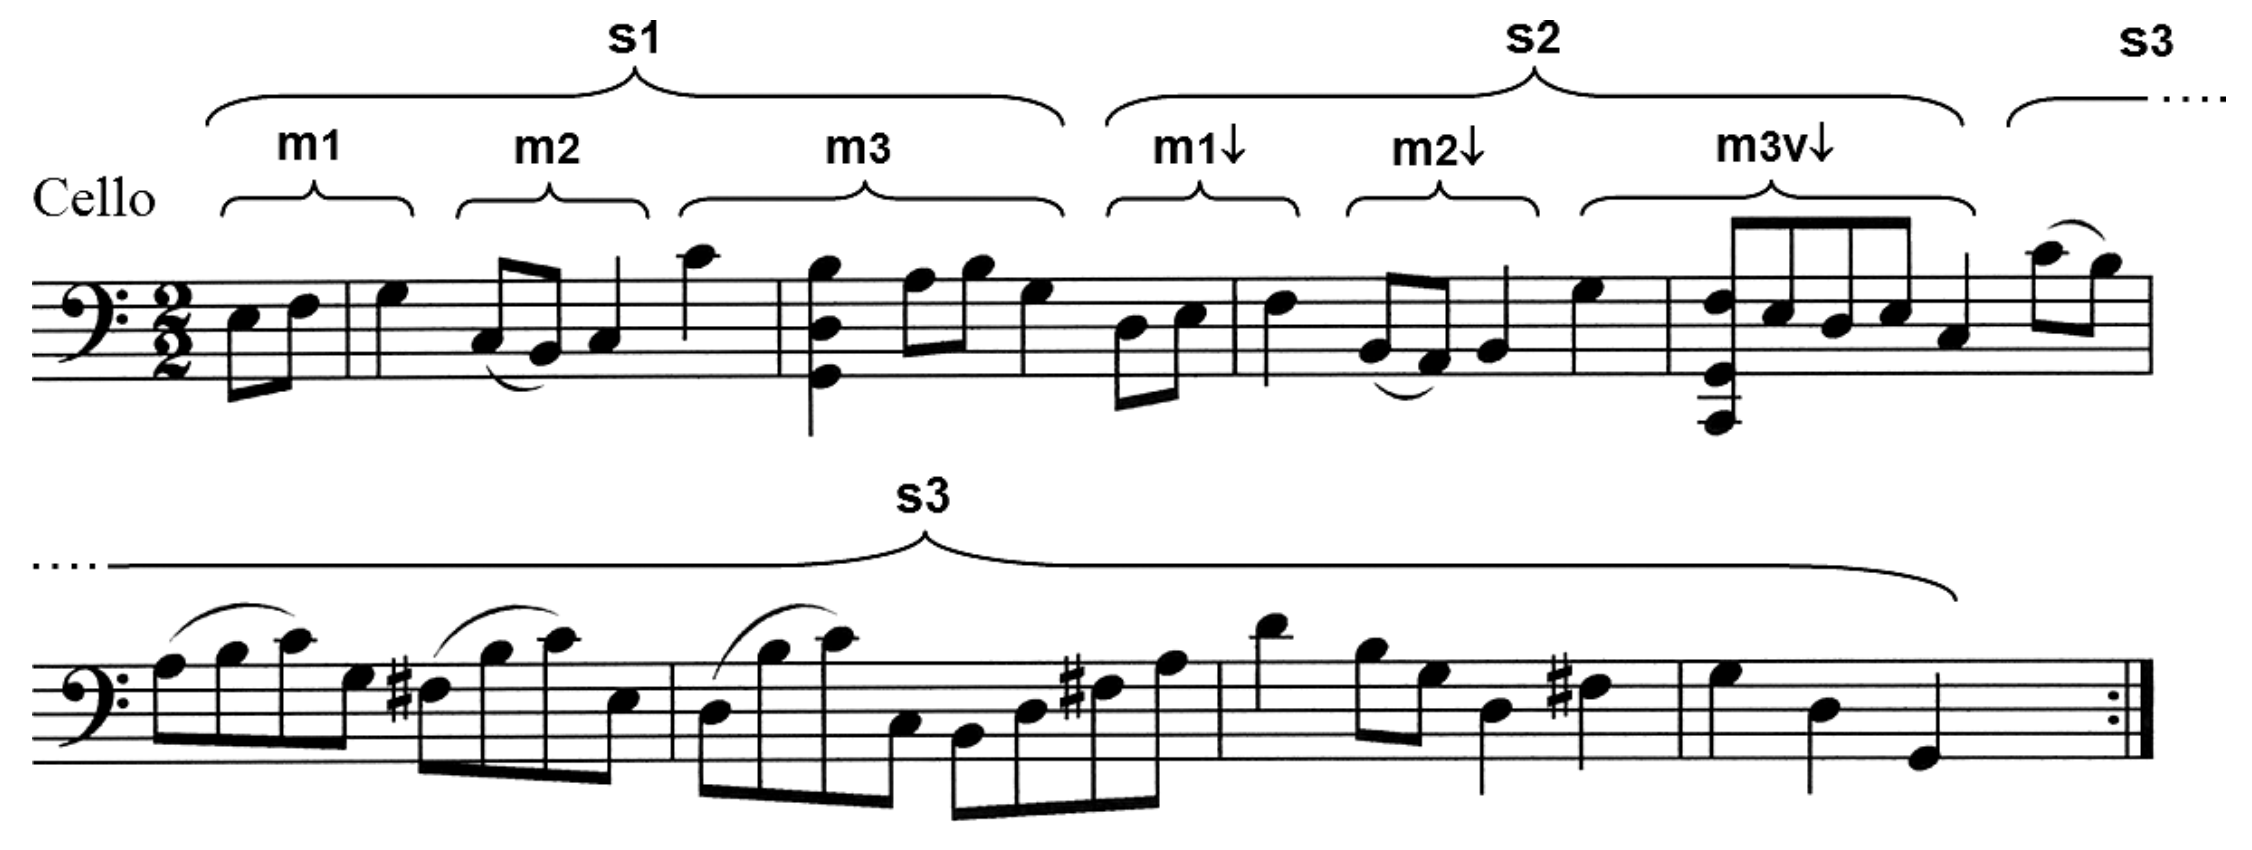
\includegraphics[width=\linewidth]{figures/bach_cello.png}
    \caption{%
        Bach Cello Suite No. 3 in C Major, V. Burrée I.
    }\label{fig:bach}
\end{figure}

There are many tales of Bach's impressive talents as a composer and virtuoso
musician. A biographer of Bach recounts that Bach arrived to the main  town in
Prussia as a “stranger”. Upon arrival King Frederick the Great invited him to
the Royal Palace to try the new pianofortes. ``After he had gone on for some
time, he asked the King to give him a subject for a Fugue, in order to execute
it immediately without any preparation.''\cite{6}. Speaking about this same event,
Douglas Hofstadter in his book Godel, Escher, Bach: An Eternal Golden Braid
states, ``the ten canons in the musical offering are among the most sophisticated
canons Bach ever wrote. However, curiously enough, Bach himself never wrote them
out in full. This was deliberate. They were posed as puzzles to King Frederick.
It was a familiar musical game of the day to give a single theme, together with
some more or less tricky hints, and to let the canon based on the theme be
`discovered' by someone else''\cite{7}. This shows that Bach truly incorporated math
into his music and that his compositions were much more than a creative thought;
that they contained a mathematical complexity that retained beauty. So, it is
possible to see that his music contained fractal.

The paper Structural Scaling of Bach’s Cello Suite No.3 by Harlan Brothers is
dedicated entirely to examining the scaling characteristics within the Bourrée
Part 1 (the score of which is displayed in Figure~\ref{bach}). The structural
scaling that Brothers noticed in his Bach’s Cello Suite No. 3 can be described
by the four figures he provided below. In the section m1 and m2 of the first
figure we see two eighth notes followed by a
quarter note. This structure of Short-Short-Long is repeated throughout this
section of the piece by Bach. The section m3 is also Short-Short-Long but scaled
twice as long as the m1, and m2 section so it contains two quarter notes
followed by a section of the duration of a half note. Since m3 is twice as long
as m2 and m1, in section s1 we again see the pattern of Short-Short-Long.
Continuing in the same manner we can see how s1, s2 and s3 form a
Short-Short-Long pattern as well. In Figure~\ref{bach_scale} we can visually see
that the self-similar pattern resembles the section as a whole in three
different levels.

\begin{figure}[ht!]
    \centering
    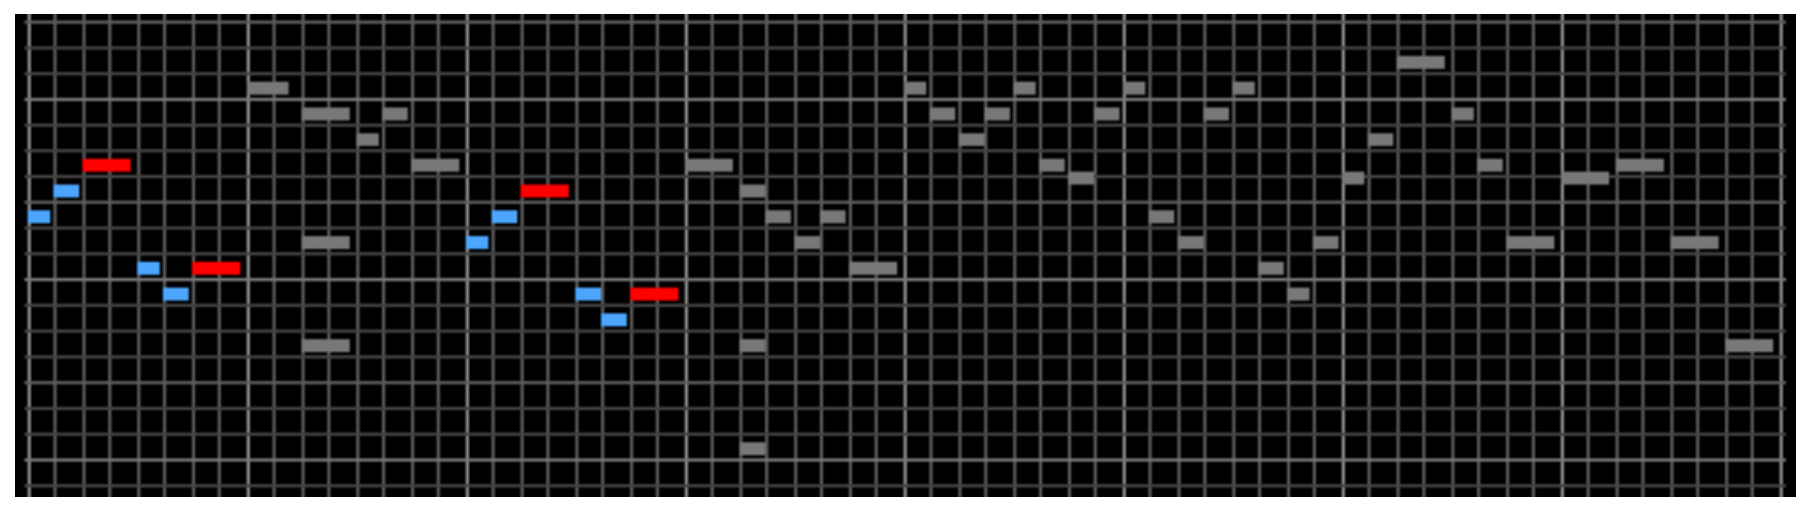
\includegraphics[width=\linewidth]{figures/bach_cello_midi01.png}
    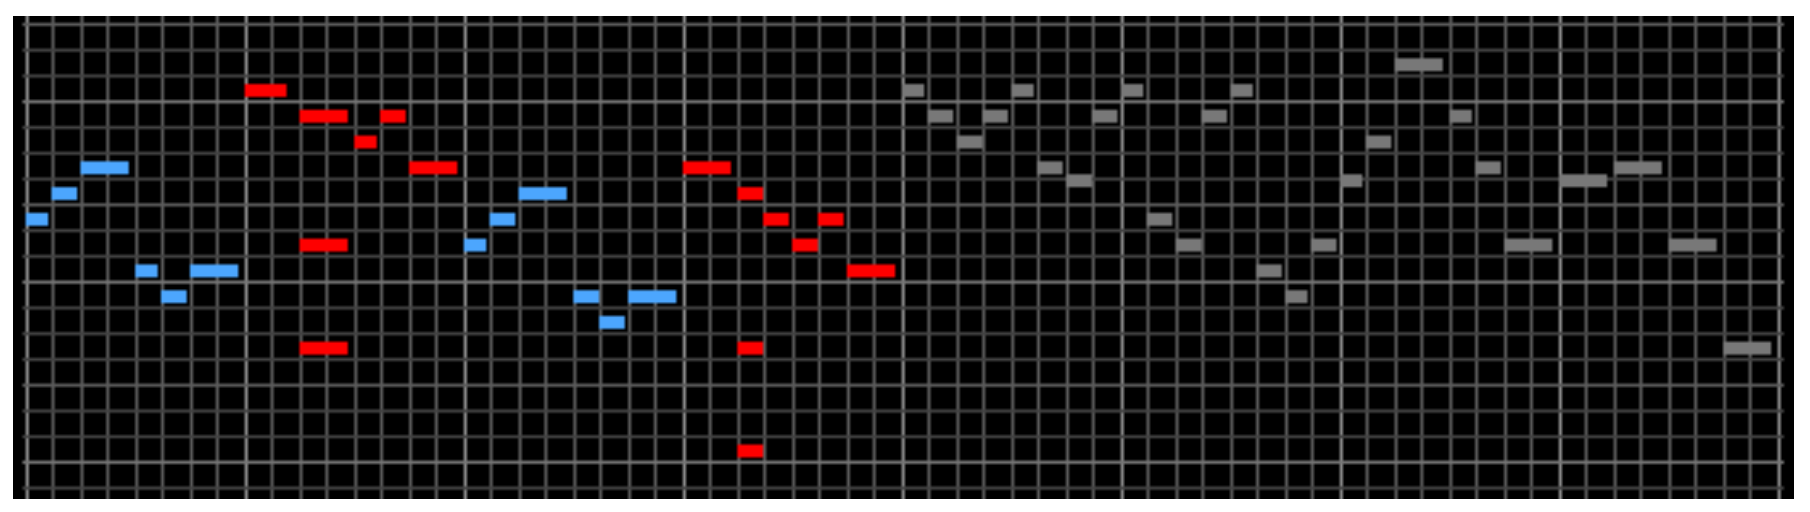
\includegraphics[width=\linewidth]{figures/bach_cello_midi02.png}
    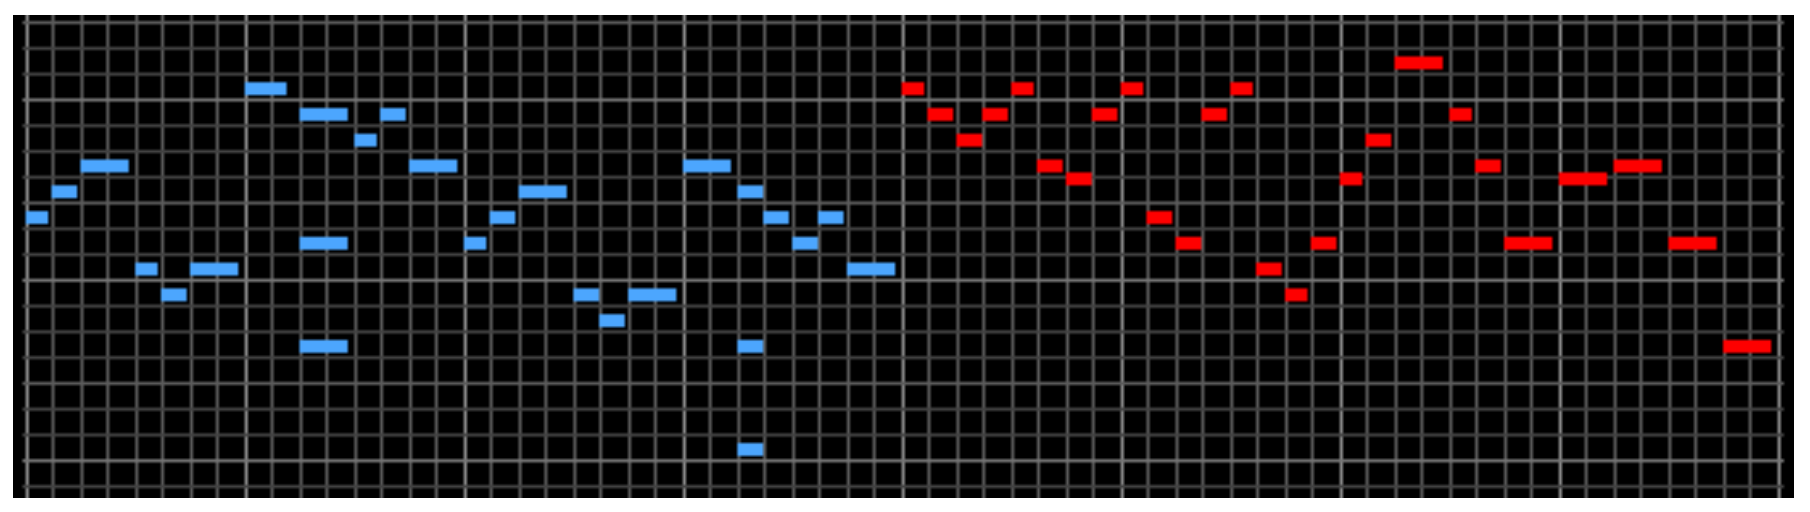
\includegraphics[width=\linewidth]{figures/bach_cello_midi03.png}
    \caption{%
        Structurally self similar patterns at different scales.
    }\label{fig:bach_scale}
\end{figure}

\section{Pitch scaling and stochastic composition}

Stochastic pitch scaling can be generated using a method that involves rolling a
number of dice, and the sum of the dice gives a note that was assigned a number.
For example 7 could be assigned to the note D. Bulmer used six dice to generate
a scale of notes that when listened to has a static like sound. The noise that
is termed for this is white noise, which music that is considered white noise
has an atrocious sound to it due to the disconnection of flow when going from
note to note. White noise is considered to be too unpredictable, where brown
noise is considered to be very predictable. Brown noise has a Brownian motion
which can be seen as being too predictable because the notes have an erratic
motion back and forth. White and brown noise are the two extremes for random
music.

Pink noise has been seen to achieve both of these extremes which brings a
balance which is considered the $\sfrac 1 f$ noise\cite{1}. Achieving a true balance
between these extremes is very difficult, as described by Mandelbrot (1971)[8,9].
Pink noise has been seen to have a self-similar process with a pattern that is
long-range dependent and exhibits short-term randomness.

Voss approximates pink noise using a variation of the dice method that was
described earlier. Using $n$ dice, for our experiment we used $n=3$, we generated
$2^{n}$ notes. The table below was constructed by rolling three dice that are
labeled A, B, and C. We sum of the three dice and the total gave us a note which
each note was assigned to a value. Binary digits were used to generate the next
note which changes from row to row in the table. The table below is the results
from our experiment. The notes below provide a stability in the sequence while
having long-range dependence which is needed to be considered pink noise.

\begin{center}
    \begin{tabu}{ccccc}
        A & B & C & Total & Note \\
        \toprule
        2 & 6 & 1 & 9     & C \\
        2 & 6 & 5 & 13    & G \\
        2 & 2 & 5 & 9     & C \\
        2 & 6 & 2 & 10    & D \\
        4 & 6 & 2 & 12    & F \\
        1 & 6 & 3 & 10    & D \\
        2 & 4 & 3 & 9     & C \\
        6 & 2 & 1 & 9     & C
    \end{tabu}
\end{center}

\begin{figure}[ht!]
    \centering
    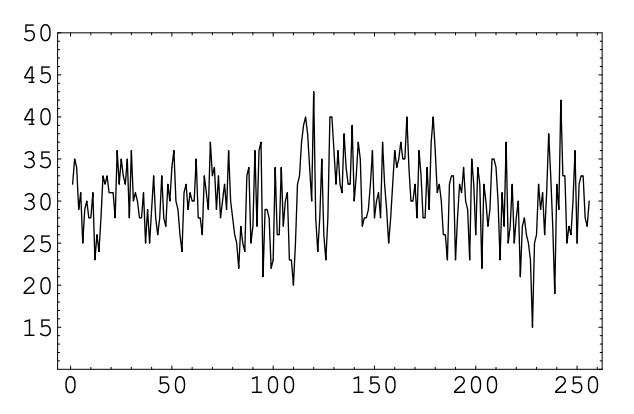
\includegraphics[width=\linewidth]{figures/pink_noise_time.png}
    \caption{%
        Time plot of pink noise\cite{8}
    }\label{fig:pink_t}
\end{figure}

Figure~\ref{fig:pink_t} shows a time plot produced using the dice method created
by Voss, we are able to see that the series of notes exhibit long-range
dependence. There is more stability due to the high digits have less change.

When describing noise we can use autocorrelation to describe the notion of music
notes being ``related'' over time. Autocorrelation is composed of two data sets,
$r$, which is the values in the noise sequence and $k$ which is called the lag.

\[
    r_k=\frac
    {\sum_{t=1}^{N-k} (x_t-\bar x)(x_{t+k}-\bar x)}
    {\sum_{t=1}{N}{(x_t-\bar x)}^2}
\]

The formula above can be used to construct correlograms, a plot of
autocorrelation against lag. This will give a visual into the autocorrelation
structure of the noise.

\begin{figure}[ht!]
    \centering
    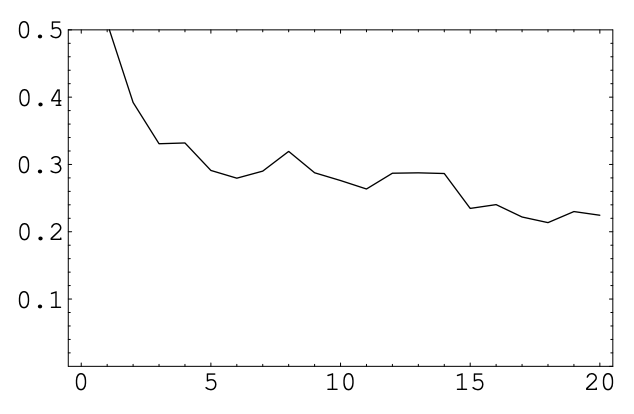
\includegraphics[width=\linewidth]{figures/pink_noise_correlogram.png}
    \caption{%
        Correlogram for pink noise\cite{8}
    }\label{fig:pink_c}
\end{figure}

Figure~\ref{fig:pink_c} shows that within the correlation over time does
not disappear to even over a longer period of time. Pink noise exhibits the 1/f
phenomena which is attributed to the pitch scaling. We can see that that the
extremes of pitch scaling can lead to some dissonance in sounds. When finding a
balance in the scaling the results can begin to exhibit fractal characteristics.
The compositions of songs are reminiscent of the Koch snowflake which possesses
long-range dependence and short-term randomness which was observed in pink
noise. The results is a composition that is self-similar which like snowflakes
are considered fractals.

\section{Melodic interval and duration scaling}

In their article “Multifractal analyses of music sequences”\cite{12}, Zhi-Yuan Su and
Tzuyin Wu concerned themselves with the analysis of music using two of the seven
previously mentioned methods of structural scaling: melodic interval scaling and
duration scaling. Following a summary of music as 1/f noise and fractal geometry
in music as described by the literature of authors like Mandelbrot and duo Voss
and Clarke, authors Su and Wu note that many previous investigations of scaling
exponents refer only to “mean” properties of musical sequences. However, they
argue that fractal geometries are rarely accurately characterized by any single
scaling exponent, that fractal geometries and phonomena change and develop
throughout a piece of music, and that such clustering patterns are certainly not
uniform. A more granular approach was necessary. The authors loosely define a
“multifractal” as “an interwoven set constructed from sub-sets with different
local fractal dimensions”\cite{12}. Su and Wu provide a formalization of the local
scaling exponent of a point distribution (the Hölder exponent) $\alpha$ given by
the equation

\[
    \alpha = \lim_{r\to 0}\frac{\log p_i(r)}{\log r}.
\]

Where $r$ is the width of sub-covers of the point distribution and $p_i(r) =
N_i(r)/N$ the portion of points that fall within the ith sub-cover. The
generalized dimension of this point distribution is given by

\[
    D_q = \frac{1}{q-1}\lim_{r\to 0}\frac{\log\sum_i {p_i(r)}^q}{\log r}
\]

For $q$ is a given weight (or moment in terms of the exponent). They note that
common approaches to calculating the local Hölder exponent first calculate the
generalized dimension and utilize a relation between the generalized dimension
$D_q$ and $q$ via a Legendre transformation. However, for signals which are
sampled or discrete this method fails, as $D_q$ must be a smooth function.
Instead the multifractal spectrum $f(\alpha)$ can be obtained directly from the
weighted $p_i(r)$ as per the following equations

\begin{gather*}
    \mu_i(r,q) = {p_i(r)}^q / \sum_i {p_i(r)}^q \\
    \alpha(q) = \lim_{r\to 0}\frac{\sum_i \mu_i(r,q)\log p_i(r)}{\log r} \\
    f(q) = \lim_{r\to 0}\frac{\sum_i \mu_i(r, q)\log\mu_i(r,q)}{\log r}.
\end{gather*}

Following these formal descriptions, Su and Wu describe an entire methodology
for analyzing the multifractal spectrum of melodic musical passages by
converting the notes of the passage into two point sequences: one from the
absolute intervals between sequential notes, and one from the relative rhythmic
values of each note.

\subsection{Melodic interval sequence}

The first note of the passage becomes the first point of a sequence of integers
with value zero. The second point of the sequence then is the absolute value of
the intervallic distance between the first and second notes of the piece in
terms of semitones, plus the value of the previous, plus one (in the case that
two neighboring notes are actually the same note). As in the example from the
music primer, the interval from F to B consists of 6 semitones, thus the
absolute intervallic distance in either direction (from F to B or from B to F)
is 6 semitones. Repeating this process for the entirety of the passage we
generate the point sequence of integers corresponding to absolute intervallic
distance we desire. We can then consider these values to be the integer
positions on a numberline at which our points sit, and thus we generate a
sequence of points upon which we can measure sub-coverings.

As an example consider a passage of three notes, “F B C”. The first value is
always zero, the second is $6+0+1=7$, and the last is $1+7+1=9$ (B to C is a
single semitone distance). Thus we have a sequence of points at 0, 7 and 9.

\subsection{Rhythmic sequence}

For the construction of the rhythmic sequence. For our sequence of points, we
mark the 0 position as the starting point. Then we determine the shortest note
duration of the entire passage. We then divide the rhythmic value of every note
in the passage by this shortest duration. Then similar to the interval sequence,
every successive value accumulates the values of those that came before it. And
finally these values become positions with the sequence of points.

As an example consider a passage of two quarter notes and two eighth notes. We
start with 0, and find eighth notes to be the smallest rhythmic value. Two
eighth notes divide a quarter note, so the first quarter note is mapped to
$\frac{\sfrac 1 4}{\sfrac 1 8}+0=2$. Similarly the second quarter note is mapped
to 4, and then the eighth notes are mapped to 5 and 6. Thus we have a sequence
of points at 0, 2, 4, 5 and 6.

\subsection{Local Hölder exponent calculation}

Going forward, the point sequence used is generically either the melodic
interval sequence or the rhythmic sequence. Since both are simply sequences of
integer points on a numberline the process is identical. The general method of
obtaining the scaling exponent is very similar to the methods of determining the
box-counting dimension within the material of the class. We determine a range of
values for $r$, the width of sub-coverings, from 2 to one-tenth of $N$ the total
length of the sequence. Given a center position $i$ on the sequence we count the
number of points lying within an open ball of radius $r$ at the ith position.
The local Hölder exponent $\alpha$ is determined to be the slope of a linear
fitting of data points given by  $\log r$ versus $\log p_i(r)$. We then vary $i$
within the middle $\sfrac{1}{10}$ to $\sfrac{9}{10}$ portion of the sequence to
determine the variation of the local Hölder exponent for different localities
within the sequence.

\subsection{Reproduction of results}

\subsection{Limitations of the method}

The most dramatic limitation of this procedure and this metric of scaling in
general is that it requires the musical material to be monophonic---only one
note at a time---while the vast majority of modern music (and actually the
majority of music since the 14th century) is polyphonic. Despite this, a piece
of music containing simultaneous notes across simultaneous voices could
potentially be reconstructed into standalone parts, where each roughly functions
as standalone piece consisting of only a monophonic melody. Think of a Bach
cantata for soprano, alto, tenor and bass four-part choir, where each voice is
essentially its own piece, its own melody. On the other hand, not all music can
be so simply reconstructed into parts. Even the Bach selection examined by Su
and Wu (the Bourrée), despite being almost entirely monophonic, contains
polyphony in measures 2, 4, and 28 (the last), but this may be an artifact of
the editor, as some copies have a single G instead of the E chord. Either way,
one can simplify a polyphonic melody by selecting a single constituent note
whenever there's a simultaneous group of notes, as I did for simplifying the
Bourrée.

\section{Conclusions}

\begin{thebibliography}{9}
\bibitem{1}
    R. F. Voss and J. Clarke,
    ``$\sfrac 1 f$ noise in music and speech'',
    Nature Vol. 258, 1975; pp. 317--318.
\bibitem{2}
    H. J. Brothers,
    ``Structural scaling in Bach's cello suite no. 3.''
    Fractals, Vol. 15, No. 1, 2007; pp. 89--95.
\bibitem{3}
    MIT Video Production.
    ``Benoit B. Mandelbrot, MIT 2001---Fractals in Science, Engineering and Finance (Roughness and Beauty)'',
        YouTube, Jan. 17, 2019 [Video file],
    accessed Dec. 10, 2019.
    \url{https://www.youtube.com/watch?v=ock9Gk_aqw4}.
\bibitem{4}
    TED.\
    ``Fractals and the art of roughness'',
    TED, Fed, 2010 [Video file],
    accessed: Dec. 10, 2019.
    \url{www.ted.com/talks/benoit_mandelbrot_fractals_and_the_art_of_roughness/discussion}.
\bibitem{5}
    H. Brothers,
    ``Fractal Music: Common Errors.''
    \url{http://www.brothers technology.com/fractal-music/errors.html}
\bibitem{6}
    H.T. David and A. Mendel,
    The Bach Reader; pp. 305--306.
\bibitem{7}
    D.R. Hofstadter,
    \emph{Godel, Escher, Bach: An Eternal Golden Braid} (Basic Books, 1980).
\bibitem{8}
    M. Bulmer,
    ``Music From Fractal Noise''
    Proceedings of the Mathematics 2000 Festival, Melbourne, Jan 13, 2000.
\bibitem{9}
    Mandelbrot, B. (1971),
    ``A Fast Fractional Gaussian Noise Generator''.
    Water Resources Research, 7; pp. 543–553.
\bibitem{10}
    Chatfield, C. (1996),
    ``The Analysis of Time Series: An Introduction'' (4th ed.).
    London: Chapman \& Hall.
\bibitem{11}
    H. Brothers,
    ``Fractal Music: Prerequisites for fractal classification'', HTML.\
    \url{http:// www.brotherstechnology.com/yale/FractalMusic/FracMusicBground/Frac}.
\bibitem{12}
    Zhi-Yuan Su and Tzuyin Wu,
    ``Multifractal analyses of music sequences'',
    Physica D 221, 2006.
\end{thebibliography}
\end{document}
